\section{Operatori}

\begin{frame}{Iniziamo con qualche semplice operazione}
	\begin{columns}
		\begin{column}{4cm}
			\begin{figure}
   				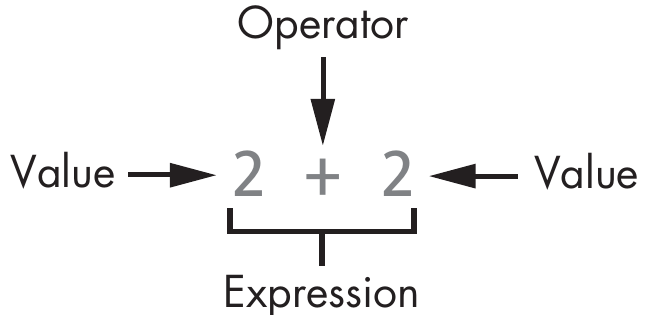
\includegraphics[height=2cm]{images/operatore_espressione.png}
			\end{figure}
		\end{column}
		\begin{column}{6cm}
            \begin{itemize}
                \item  6 + 6
                \item  7 - 5
                \item  8 / 4
                \item  9 * 3
                \item 12.5 * 3 cosa c'è di diverso qui?
                \item  (2 + 3 - 4) * 5 / 6 
            \end{itemize}
		\end{column}
	\end{columns}
\end{frame}

\begin{frame}{Iniziamo con qualche semplice operazione}
	\begin{columns}
		\begin{column}{4cm}
			\begin{figure}
   				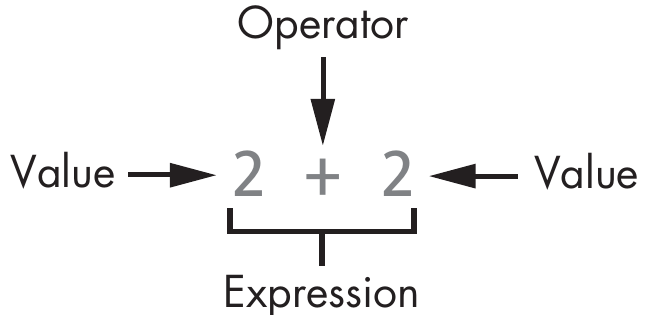
\includegraphics[height=2cm]{images/operatore_espressione.png}
			\end{figure}
		\end{column}
		\begin{column}{6cm}
            \begin{itemize}
                \item  6 + 6
                \item  7 - 5
                \item  8 / 4
                \item  9 * 3
                \item 12.5 * 3 cosa c'è di diverso qui?
                \item  (2 + 3 - 4) * 5 / 6 
            \end{itemize}
		\end{column}
	\end{columns}
	
	\begin{block}{Cosa succede se sbaglio a scrivere?}
	    5 +
	    
	    \lstinline{Syntax Error: Invalid syntax}
	\end{block}
\end{frame}